\section{The Bott and Chern Markers}
\label{sec:bott_chern}

Let us start with the Bott index, initially proposed by Hastings and Loring~\cite{hastings_almost_2010,hastings_topological_2011}. This marker is most naturally suited to systems in periodic boundary conditions. This section is as follows: We derive the exact form of the Bott index, showing that it is exactly equal to Chern number in a periodic, translationally symmetric system. In \textsection\ref{sec:chern_marker} we show how the Chern marker~\cite{bianco_mapping_2011} (also given by Kitaev in Eqn.~\ref{eqn:chern_marker_from_kitaev}) can be understood as the Bott index in the large-system limit.

We will work with a lattice model, where unit cells are indexed by a vector of the form $(m_x,m_y)$. The lattice has size $(L_x,L_y)$, and we have set periodic boundary conditions. Sites are indexed by 
\begin{align}
	\ket{\textbf m \alpha} = \ket{\textbf m} \otimes \ket{\alpha},
\end{align} 
where $\textbf m$ is a vector labelling the unit cell and $\alpha$ selects a site within the unit cell. We shall use a Hamiltonian that has translational symmetry, so we may apply Bloch's theorem to obtain the form of the energy eigenstates,
\begin{align}
	 H &= \sum_{\textbf k} \ket{\textbf k}\bra{\textbf k}\otimes  H(\textbf k) \\ 
	\ket{\psi_{\textbf k, n}} &= \ket{\textbf k} \otimes\ket {u_{\textbf k, n}},
\end{align}
where $\ket {u_{\textbf k, n}}$ are the eigenstates of $ H(\textbf k)$ and the momentum states are defined as in Eqn.~\ref{eqn:k_state_def}. We assume that the system has a total of $\eta$ bands, so $n \in  \{1,...,\eta\}$. Henceforth, we will assume that only the $n$\ts{th} band is occupied, so we can construct a projector onto the occupied subspace, $ P$, and its complement, $ Q$.
\begin{align}
	 P & = \sum_{\textbf k} \ket{\psi_{\textbf k, n}}\bra{\psi_{\textbf k, n}} \\
	 Q & = \sum_{\textbf k,\, m \neq n} \ket{\psi_{\textbf k, m}}\bra{\psi_{\textbf k, m}}.
\end{align}
We also introduce a pair of operators $e^{i \delta_x  x}$ and $e^{i \delta_y  y}$, 
with
\begin{align}
\delta_x = \frac{2\pi}{L_x} ,\  \delta_y = \frac{2\pi}{L_y}.
\end{align}
In order to understand the effect of these operators, we consider their effect on the plane wave states
\begin{align}
	e^{i \delta_x  x}\ket{\textbf k} &= \frac{1}{\sqrt{L_x L_y}} \sum_{\textbf m} e^{i \delta_x  x} e^{i \textbf m \cdot \textbf k} \ket {\textbf m} \\
	& = \frac{1}{\sqrt{L_x L_y}} \sum_{\textbf m} e^{i \textbf m \cdot (\textbf k + \boldsymbol{\delta}_x)} \ket {\textbf m}\\
	& = \ket{\textbf k + \boldsymbol \delta_x},
\end{align}
with a similar expression for $e^{i \delta_y  y}$. Here the symbols $\boldsymbol{\delta}_x$ and $\boldsymbol{\delta}_y$ represents a vector translation in $\textbf k$-space,
\begin{align}
	\boldsymbol \delta_x = \begin{pmatrix}
	\delta_x \\
	0
	\end{pmatrix}, \ \boldsymbol \delta_y = \begin{pmatrix}
	0 \\
	\delta_y
	\end{pmatrix}.
\end{align}
Thus, these operators effect a translation in $\textbf k$ space by the minimum step in the reciprocal lattice. Now let's look at the effect of these operators on the projector $ P$,
\begin{align}
	e^{i \delta_x  x}  P e^{-i \delta_x  x}  
	&=  \sum_{\textbf k} e^{i \delta_x  x}  \ket{\textbf k} \bra{\textbf k} e^{-i \delta_x  x}\otimes \ket{u_{\textbf k, n}}\bra{u_{\textbf k, n}} \\
	&=  \sum_{\textbf k} \ket{\textbf k +\boldsymbol{\delta}_x} \bra{\textbf k +\boldsymbol{\delta}_x } \otimes \ket{u_{\textbf k, n}}\bra{u_{\textbf k, n}} \\
	&=  \sum_{\textbf k} \ket{\textbf k } \bra{\textbf k } \otimes \ket{u_{\textbf k-\boldsymbol{\delta}_x, n}}\bra{u_{\textbf k-\boldsymbol{\delta}_x , n}},
\end{align}
where the last line follows from a redefinition of $\textbf k$. For the sake of clarity later on, we will re-express the density operator $\ket{u_{\textbf k, n}}\bra{u_{\textbf k, n}}$ in the following form
\begin{align}
	\ket{u_{\textbf k, n}}\bra{u_{\textbf k, n}} =  u_{\textbf k, n},
\end{align}
so we get
\begin{align} \label{eqn:p_identity}
	e^{i \delta_x  x}  P e^{-i \delta_x  x}  =  \sum_{\textbf k} \ket{\textbf k } \bra{\textbf k } \otimes  u_{\textbf k-\boldsymbol{\delta}_x, n}.
\end{align}
Now we have enough tools to introduce the definition of the Bott index!
\begin{align}\label{eqn:bott_index}
    B(\textbf r) =
	-\frac{N}{2\pi} \Im 
	\tr_{\textbf r} \log \left [  U V U^\dag  V^\dag +  Q \right ].
\end{align}
Here $N$ denotes the total number of unit cells in the system, $\tr_{\textbf r}$ is a local trace over the unit cell at position $\textbf r$, and the log is the matrix logarithm. The operators $U$ and $V$ are given by
\begin{align}
	 U  =  P e^{i \delta_x  x}  P, \\
	 V  =  P e^{i \delta_y  y}  P.
\end{align}
To make sense of this expression, let us focus on the $  U V U^\dag  V^\dag$ part only, writing this out explicitly gives us
\begin{align}
	  U V U^\dag  V^\dag =  P e^{i \delta_x  x}  P e^{i \delta_y  y}  P e^{- i \delta_x  x}  P e^{-i \delta_y  y}  P.
\end{align}
We now add in identities of the form $e^{i \delta_x  x} e^{-i \delta_x  x} $ and regroup the equation, taking advantage of the fact that $x$ and $y$ commute,
\begin{align}
	U V U^\dag  V^\dag =   P
	\left [ 
		e^{i \delta_x  x}  P e^{-i \delta_x  x} 
	\right ]
	\left [ 
		e^{i \delta_y  y} e^{i \delta_x  x}  P  e^{-i \delta_y  y} e^{- i \delta_x  x } 
	\right ]
	\left [ 
		e^{i \delta_y  y}  P e^{-i \delta_y  y } 
	\right ]
	P.
\end{align}
Using Eqn.~\ref{eqn:p_identity} we can now rewrite this in terms of Bloch states to get
\begin{align}
	 U V U^\dag  V^\dag = \sum_{\textbf k} \ket{\textbf k } \bra{\textbf k } \otimes   u_{\textbf k, n}   u_{\textbf k -\boldsymbol{\delta}_x , n}   u_{\textbf k-\boldsymbol{\delta}_x-\boldsymbol{\delta}_y, n}   u_{\textbf k-\boldsymbol{\delta}_y, n}   u_{\textbf k, n}.
\end{align}
Since the first and last $ u$ density operator in this expression are identical, we can rewrite this in terms of a trace to get
\begin{align}
	 U V U^\dag  V^\dag = \sum_{\textbf k} \ket{\textbf k } \bra{\textbf k } \otimes  \ket {u_{\textbf k, n}} \bra{u_{\textbf k, n}} \cdot  \tr \left [  u_{\textbf k, n}  u_{\textbf k -\boldsymbol{\delta}_x , n}   u_{\textbf k-\boldsymbol{\delta}_x-\boldsymbol{\delta}_y, n}   u_{\textbf k-\boldsymbol{\delta}_y, n} \right ].
\end{align}
If we compare this to the definition of Berry flux (Eqn.~\ref{eqn:berry_flux}), we see that we have exactly constructed an inner product of a loop of adjacent states on the Brillouin zone, and this reduces to
\begin{align}
	 U V U^\dag  V^\dag = \sum_{\textbf k} \ket{\textbf k } \bra{\textbf k } \otimes  \ket {u_{\textbf k, n}} \bra{u_{\textbf k, n}} \cdot r_{\textbf k} e^{-i F_{\textbf k-\boldsymbol{\delta}_x-\boldsymbol{\delta}_y}},
\end{align}
where $r_{\textbf k}$ is just some real number that we don't care about, arising from adjacent $u$ states not having a perfect overlap. Since we are aiming to get a sum of $F_{\textbf k}$ over the whole Brillouin zone, let us take the logarithm of this matrix
\begin{align}
	\log \left [  U V U^\dag  V^\dag +  Q \right ] = \sum_{\textbf k} \ket{\textbf k } \bra{\textbf k } \otimes  \ket {u_{\textbf k, n}} \bra{u_{\textbf k, n}}
	\left ( \log(r_{\textbf k})-i F_{\textbf k-\boldsymbol{\delta}_x-\boldsymbol{\delta}_y}\right ),
\end{align}
where we have added the projector onto the unoccupied subspace to ensure it does not diverge. Finally, let us select some arbitrary unit cell in our system at position $\textbf r$ and take a local trace, 
\begin{align}
	\tr_{\textbf r}
	\log \left [  U V U^\dag  V^\dag +  Q \right ]   
	= \sum_{\textbf k} 
	|\braket{\textbf r|\textbf k}|^2 
	\braket{u_{\textbf k, n}|u_{\textbf k, n} }  
	\left ( 
		\log(r_{\textbf k})-i F_{\textbf k-\boldsymbol{\delta}_x-\boldsymbol{\delta}_y}
	\right ).
\end{align}
We can show that $|\braket{\textbf r|\textbf k}|^2 = \frac{1}{N}$ and $\braket{u_{\textbf k, n}|u_{\textbf k, n} } = 1$. All that is left to do is take the imaginary part, 
\begin{align}
	\Im 
	\tr_{\textbf r}
	\log \left [  U V U^\dag  V^\dag +  Q \right ]   
	= \frac{1}{N} \sum_{\textbf k} - F_{\textbf k-\boldsymbol{\delta}_x-\boldsymbol{\delta}_y} .
\end{align}
Now, redefining $\textbf k$ and adding back in the factor of $-\frac{N}{2\pi}$ gives us
\begin{align}
	-\frac{N}{2\pi} 
	\Im 
	\tr_{\textbf r}
	\log \left [  U V U^\dag  V^\dag +  Q \right ].
	= \frac{1}{2\pi} \sum_{\textbf k}  F_{\textbf k}.
\end{align}
By comparing with Eqn.~\ref{eqn:discrete_chern_number}, we can see that we have arrived at an expression for the Chern number!
\begin{align}
	\mathcal Q = -\frac{N}{2\pi} 
	\Im 
	\tr_{\textbf r}
	\log \left [  U V U^\dag  V^\dag +  Q \right ].
\end{align}
Thus, we have shown that in the case of a translationally symmetric system with periodic boundaries, the Bott index evaluated at any point in our material always exactly calculates the Chern number.

\subsection{The Chern Marker} \label{sec:chern_marker}

Most sources cite~\cite{bianco_mapping_2011} for the invention of the Chern marker, however as we shall see in \textsection\ref{sec:kitaev_marker}, the Chern marker is a relatively trivial restatement of Kitaev's marker. Here we will derive the Chern marker by showing that it can be obtained from the Bott index in the limit of large system size.

Our starting point is the expression for Bott index, Eqn.~\ref{eqn:bott_index}, which we rewrite using the following shorthand
\begin{align}
	P_x &= e^{i\delta_x x} P e^{-i\delta_x x},\\
	P_y &= e^{i\delta_y y} P e^{-i\delta_y y},\\
	P_{xy} &= e^{i\delta_x x +i\delta_y y} P e^{-i\delta_x x - i\delta_y y}.
\end{align}
Thus, the Bott index can be written as
\begin{align}
	B(\textbf r) = - \frac{N}{2\pi} \im \tr_{\textbf r} \log \left [ 
		P P_x P_{xy} P_y P + Q
	\right ].
\end{align}
Now let us expand the translated projectors in $\delta$,
\begin{align}
	P_x &= P +i\delta_x [x,P] \\ 
	P_y &= P +i\delta_x [y,P] \\ 
	P_{xy} &= P +i\delta_x [x,P]+i\delta_y [y,P].
\end{align}
Thus, the term in the trace can be expanded up to second order as
\begin{align}
	P P_x P_{xy} P_y P + Q = \1 - 2 \delta_x \delta_y
	P[x,P][y,P]P + ... + \mathcal O(\delta^3),
\end{align}
where we have used the identity $P[P,O]P = 0$ for any $O$, and `...' represents two Hermitian terms of order $\delta_x^2$ and $\delta_y^2$, which vanish when the imaginary part of the trace is taken. Now let us use the identity $\log( \1 + x) \approx x$ to express the expanded Bott index as
\begin{align} \label{eqn:chern_bott_expansion}
	B(\textbf r) = - \frac{N \delta_x \delta_y} {2\pi} \tr_{\textbf r} \left (
	P[x,P][y,P]P 
	\right ) - h.c. + \mathcal O(\delta^3).
\end{align}
Now, writing explicitly the form of $\delta_\alpha$ and expanding out the commutators one arrives at
\begin{align} \label{eqn:chern_marker}
	B(\textbf r) \rightarrow C(\textbf r) = - 2\pi i \tr \left [
		PxP, PyP
	\right ],
\end{align}
which is precisely the expression for the Chern marker~\cite{bianco_mapping_2011}.

\begin{shaded}
	\textit{A Quick Note on Periodic Boundaries --- } As we shall see in the following examples, the Chern marker is ill-suited to periodic boundaries. This is because the position operators $x$ and $y$ have discontinuities at the system boundaries. However, Eqn.~\ref{eqn:chern_bott_expansion} hints at the correct way to modify the Chern marker to be well-behaved in PBC. This can be done by noticing that the commutators $[x,P]$ and $[y,P]$ effectively calculate a displacement. Expressing $P$ in the position basis, $P = \sum_{jk} P_{jk}\ketbra{x_j}{x_k}$ these commutators may be written as,
	\begin{align}
		[x, P] = \sum_{jk} P_{jk}(x_j - x_k) \ketbra{x_j}{x_k},
	\end{align}
	with a similar expression for $[y,P]$. If $x_j$ and $x_k$ are on opposite sides of the `stitch' in the boundary conditions, where $x$ is discontinuous then this displacement will be incorrect. Thus, we may fix this by ensuring that the displacements are always calculated using the shortest distances \textit{in period boundary conditions}. 
	\begin{align}
		[x, P]_{PB} = \sum_{jk} P_{jk} \Delta_{x, jk} \ketbra{x_j}{x_k},
	\end{align}
	where $\Delta_{x, jk}$ is the shortest displacement from point $j$ to point $k$ in PBC. Of course this will only work when $P$ is short-ranged compared to the system size, since this argument only makes sense when we are finding the displacement between two points that are relatively close to one another, ensuring that the shortest path from $i$ to $j$ is obvious. In general, this is true in any region where the system is locally gapped, which we discuss further in \textsection\ref{sec:kitaev_marker} \cite{hastings_spectral_2006}.
	
	Thus, a version of the Chern marker that is well-behaved in PBC is given by 
	\begin{align}  \label{eqn:pbc_chern_marker}
		C_{PB}(\textbf r) = - 2\pi \tr_{\textbf r} 
		\left (
		P[x,P]_{PB}[y,P]_{PB}P 
		\right ) 
		- h.c.
	\end{align}
\end{shaded}

\subsection{Some Examples}

\begin{figure}
    \centering
     \begin{center}
        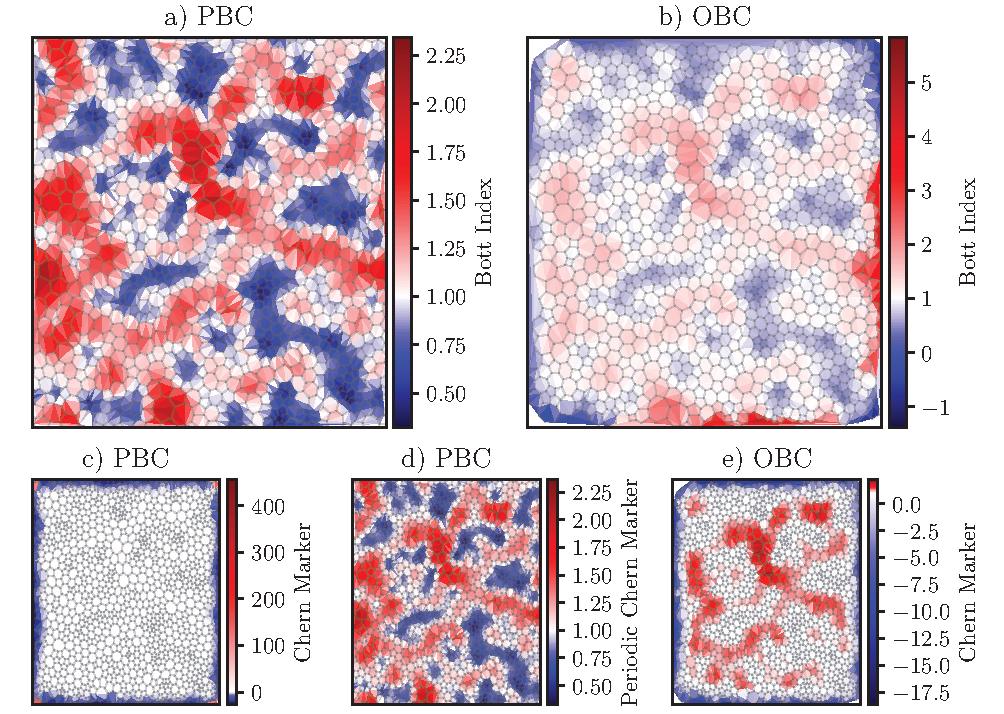
\includegraphics[width = \textwidth]{crosshair_marker/figures/markers_example.pdf}
    \end{center}
    \captionof{figure}[Bott index and Chern marker for a sample of amorphous QWZ model.]{
    Bott index and Chern markers calculated for an example amorphous QWZ model with $u=-0.5$.
	\textbf{(a)}~The Bott index calculated in periodic boundary conditions (PBC). 
	\textbf{(b)}~The Bott index calculated in open boundary conditions (OBC). Here we see sharp drops on some edges and a large spike localised on two edges, and in the bulk an identical profile as in subplot (a).
	\textbf{(c)}~The Chern marker calculated according to Eqn.~\ref{eqn:chern_marker} in PBC. The bulk variation in the marker is barely visible due to the large discontinuities at the boundaries of the material, where the $x$ and $y$ operators are discontinuous. 
	\textbf{(d)}~The modified periodic Chern marker calculated according to Eqn.~\ref{eqn:pbc_chern_marker} in PBC. Here the boundary discontinuities vanish, and the marker is almost identical to the Bott index in subplot (a).
	\textbf{(e)}~The Chern marker calculated according to Eqn.~\ref{eqn:chern_marker} in OBC. Here the marker must sum to zero, which leads to the presence of sharp drops at the boundaries, counteracting the positive bulk value.
    }\label{fig:marker_examples}
\end{figure}%

Let us finish this section by illustrating a few examples of Bott and Chern markers for an amorphous QWZ model, shown in Fig.~\ref{fig:marker_examples}. In each case we calculate the marker for the same Hamiltonian -- corresponding to the model with internal parameter $u = -0.5$ -- around the centre of the topological gap seen in Fig.~\ref{fig:amorphous_qwz_examples}b. Both the Bott index and the Chern markers have average bulk values of $+1$, verifying that this model does indeed have a nonzero topological invariant. 

In all the examples shown, the Bott index, Chern marker and periodic Chern marker have an average bulk value that corresponds to the Chern number, although there are substantial deviations around this average, which we discuss in the next subsection. Additionally, both markers display unexpected behaviour around the boundaries of the system. In the case of the Bott index, the local value around the edges of the material must be ignored, where the presence of edge modes leads to sharp positive and negative peaks. Considering the Chern marker, edge effects appear in both periodic and open boundaries, where in both cases the global sum of the Chern marker, being the trace of a commutator in a finite system, must vanish. In periodic boundaries the origin of this discontinuity of obvious, the $x$ and $y$ operators are not periodic, and have large discontinuities at the boundaries, so the marker could not be expected to be smooth at these points. Although we note that, using the `periodic Chern marker' described in Eqn.~\ref{eqn:pbc_chern_marker}, these discontinuities can be removed, providing a marker that is almost identical to the Bott index, but with the added advantage of being much less computationally expensive, since the Chern marker avoids the need for a matrix logarithm. Finally, we see that in open boundaries the Chern marker has sharp drops at the boundaries of the system which ensure that the sum over the whole system vanishes. 

\subsubsection{Are These Markers Purely Topological?}

\begin{figure}
    \centering
     \begin{center}
        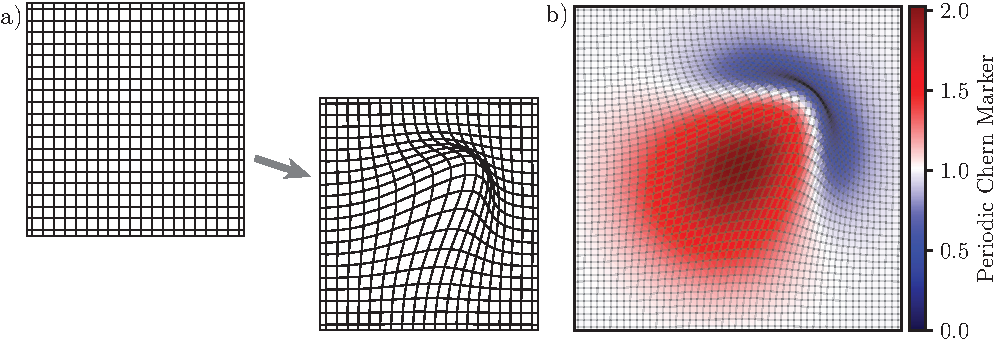
\includegraphics[width = \textwidth]{crosshair_marker/figures/lattice_warp.pdf}
    \end{center}
     \captionof{figure}[Effect of lattice-only distortion on the Chern marker or Bott index.]{
		The effect of a lattice-only distortion on the Chern marker of a translationally uniform QWZ model in PBC with $u = 0.5$ -- a system with Chern number $\mathcal Q = +1$.
		\textbf{(a)}~A lattice distortion is applied to the system, where individual sites are translated according to a Gaussian function of their position. 
		\textbf{(b)}~The Chern number is calculated using an identical Hamiltonian and projector to the undistorted, with spatial positions shifted by the lattice distortion. Where the inter-site distances have been stretched, the Chern marker is larger than the exactly known Chern number, appearing to indicate a region of Chern number $\mathcal Q =+2$. Equally, where the lattice is compressed the Chern marker is reduced, appearing to show $\mathcal Q = 0$.
    }\label{fig:lattice_warp}
\end{figure}%

Careful inspection of the examples shown in Fig.~\ref{fig:marker_examples} will reveal a peculiar structure to the deviations of the Bott and Chern markers around their bulk average (the Chern number, $+1$). In some regions the marker appears to indicate a Chern number of $+2$ and in other regions it seems to show $\mathcal Q = 0$. Thus, one might conclude that the material has a deeply complex topological structure, where pockets of different Chern numbers appear scattered throughout. This would be a mistake however, which can be seen by considering the geometry of the amorphous lattice. Areas where the marker is larger tend to correspond to regions where the plaquettes are larger and the sites are spaced further apart. Equally, dips in the value correspond to regions where the vertices are closer together. Thus, uneven spacing between vertices has the effect of overestimating the Chern number when vertices are further apart (so $\Delta x$ appears larger between sites) and underestimating it when vertices are closer together (so $\Delta x$ appears smaller between sites).

In order to illustrate this, let us consider a translationally symmetric QWZ model constructed on a square lattice with uniform $u = 0.5$. Here we expect that the Bott index or periodic Chern marker will be precisely $+1$ throughout the system. Let us consider distorting the lattice as shown in Fig.~\ref{fig:lattice_warp}a while keeping the Hamiltonian (and thus the projector $P$) invariant. Since the properties of the state itself have not changed under such a transformation, one expects the topological properties of the system to remain invariant. However, calculating the local Chern marker, as shown in Fig.~\ref{fig:lattice_warp}b, we find the value substantially inflated at points where the lattice has expanded, and vice versa at points of contraction. Thus, we see that these local markers do not solely capture the topological properties of the occupied band, but also depend on the details of the lattice embedding on the plane. Of course, averaging over a sufficiently large area one can always recover a close to quantised value. However, if we accept that such markers can only be interpreted by considering an average over a large region of the bulk then how can they be considered local? In the next section we shall present an alternative, where the Chern number is calculated around a single point in the bulk of the material, and the locality of the marker can be explicitly seen from the spatial distribution of the marker value around that point. 
